\section{Gestion des clients}

\subsection{Objectif du module}

La gestion des clients permet au fournisseur de consulter la liste des abonnés, d'afficher la fiche d'un client, d'ajouter un nouveau client, de modifier ses informations et de le supprimer lorsque les règles d'intégrité le permettent.

Le module suit l'architecture MVC :

\begin{itemize}[leftmargin=*]
  \item \textbf{Modèle} : \texttt{BD/ClientBD.php} ;
  \item \textbf{Contrôleur} : \texttt{Traitement/Client.php} ;
  \item \textbf{Vues} : \texttt{IHM/client/index.php}, \texttt{one.php}, \texttt{add.php}, \texttt{update.php} et \texttt{form.php}.
\end{itemize}

\subsection{Modèle : la classe ClientBD}

La classe \texttt{ClientBD} est la seule couche du module à contenir du SQL. Chaque méthode correspond à une opération sur la table \texttt{client} :

\begin{itemize}[leftmargin=*]
  \item \texttt{lister()} : liste les clients d'un fournisseur, avec recherche ;
  \item \texttt{trouver()} : retourne un client selon son identifiant et son fournisseur ;
  \item \texttt{creer()} : insère un nouveau client ;
  \item \texttt{mettreAJour()} : met à jour les informations d'un client ;
  \item \texttt{supprimer()} : supprime un client ;
  \item \texttt{emailExiste()} et \texttt{cinExiste()} : vérifient l'unicité ;
  \item \texttt{nbConsommations()} : compte les consommations d'un client.
\end{itemize}

Toutes les requêtes sont préparées. Les valeurs ne sont jamais concaténées directement dans le texte SQL, ce qui protège contre les injections SQL.

\subsection{Contrôleur : Traitement/Client.php}

Le contrôleur est le chef d'orchestre du module. Chaque action est une fonction :

\begin{itemize}[leftmargin=*]
  \item \texttt{client\_all()} : affiche la liste et gère la recherche ;
  \item \texttt{client\_one()} : affiche la fiche d'un client ;
  \item \texttt{client\_add()} : affiche puis traite le formulaire d'ajout ;
  \item \texttt{client\_update()} : affiche puis traite le formulaire de modification ;
  \item \texttt{client\_delete()} : supprime un client si les règles d'intégrité le permettent.
\end{itemize}

Des fonctions d'appui complètent ces actions : \texttt{client\_exiger\_fournisseur()} vérifie que l'utilisateur est un fournisseur connecté, \texttt{client\_lire\_formulaire()} nettoie et valide les champs, et \texttt{client\_csrf\_valide()} contrôle le jeton CSRF.

\subsection{Vues : IHM/client}

Les vues ne contiennent que du HTML et du PHP d'affichage. Elles ne font aucune requête SQL. Elles reçoivent leurs données du contrôleur sous forme de variables : liste des clients, fiche client, messages d'erreur ou valeurs saisies.

Le formulaire \texttt{form.php} est partagé entre l'ajout et la modification, ce qui évite de dupliquer le code. Les pages \texttt{add.php} et \texttt{update.php} fournissent le layout, le titre et la carte autour du formulaire. Toute valeur affichée est échappée avec la fonction \texttt{e()} pour empêcher les failles XSS.

\begin{figure}[htbp]
  \centering
  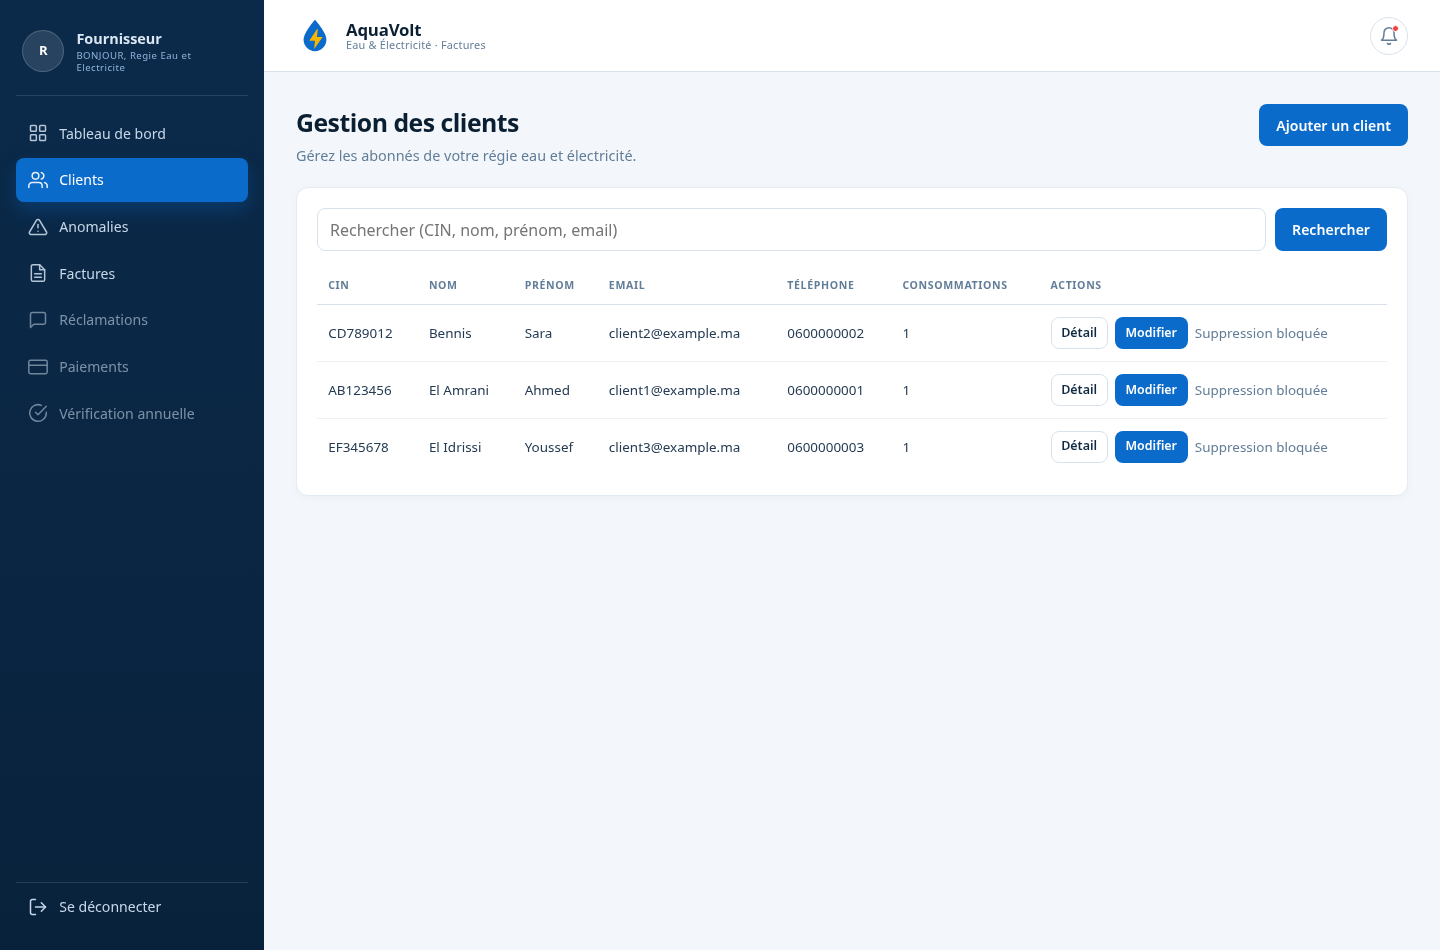
\includegraphics[width=0.72\textwidth]{figures/clients_liste.png}
  \caption{Liste des clients avec recherche}
  \label{fig:clients}
\end{figure}

\subsection{Déroulement d'une requête d'ajout}

Lorsque le fournisseur ouvre \texttt{/Client/add}, le contrôleur affiche le formulaire vide. Lors de l'envoi :

\begin{enumerate}[leftmargin=*]
  \item le contrôleur vérifie le rôle de l'utilisateur ;
  \item il vérifie le jeton CSRF ;
  \item il valide chaque champ : CIN, nom, prénom, adresse, email, téléphone et mot de passe ;
  \item il vérifie que l'email et le CIN n'existent pas déjà ;
  \item il hache le mot de passe avec \texttt{password\_hash()} ;
  \item il demande au modèle d'enregistrer le client ;
  \item il redirige vers la liste avec un message de succès.
\end{enumerate}

En cas d'erreur, il réaffiche le formulaire avec les messages et les valeurs déjà saisies. Le contrôleur ne fait jamais de SQL, le modèle n'affiche jamais de HTML et la vue ne prend aucune décision métier.

\subsection{Validation et unicité}

Les champs obligatoires sont le CIN, le nom, le prénom, l'adresse et l'email. Le CIN et l'email doivent être uniques. Le mot de passe doit contenir au moins huit caractères lors de la création. Les doublons sont détectés avant l'insertion et une contrainte d'unicité dans la base assure également l'intégrité.

La recherche porte sur le CIN, le nom, le prénom et l'email. Elle utilise une requête préparée avec des paramètres \texttt{LIKE}.

\subsection{CSRF et suppression conditionnelle}

Les formulaires d'ajout, de modification et de suppression contiennent un jeton CSRF. Le contrôleur vérifie ce jeton avant toute écriture.

La suppression est bloquée lorsqu'un client possède au moins une consommation. Le contrôleur vérifie le nombre de consommations avant de supprimer et la clé étrangère \texttt{ON DELETE RESTRICT} empêche toute suppression incohérente au niveau de la base. L'interface affiche « Suppression bloquée » à la place du bouton pour ces clients.

\subsection{Tests du module}

Les tests réalisés sur le module clients couvrent :

\begin{itemize}[leftmargin=*]
  \item l'accès à la liste et la recherche ;
  \item l'ajout d'un client valide ;
  \item le refus d'un CIN ou d'un email en doublon ;
  \item la modification des informations et du mot de passe ;
  \item le blocage de la suppression d'un client ayant des consommations ;
  \item le contrôle du rôle fournisseur et du jeton CSRF.
\end{itemize}
